\section{Kwadratury elementarne}
%%%%%%%%%%%%%%%%%%%%%%%%%
	\begin{frame}{Wzór prostokątów}
      	\begin{center}
      		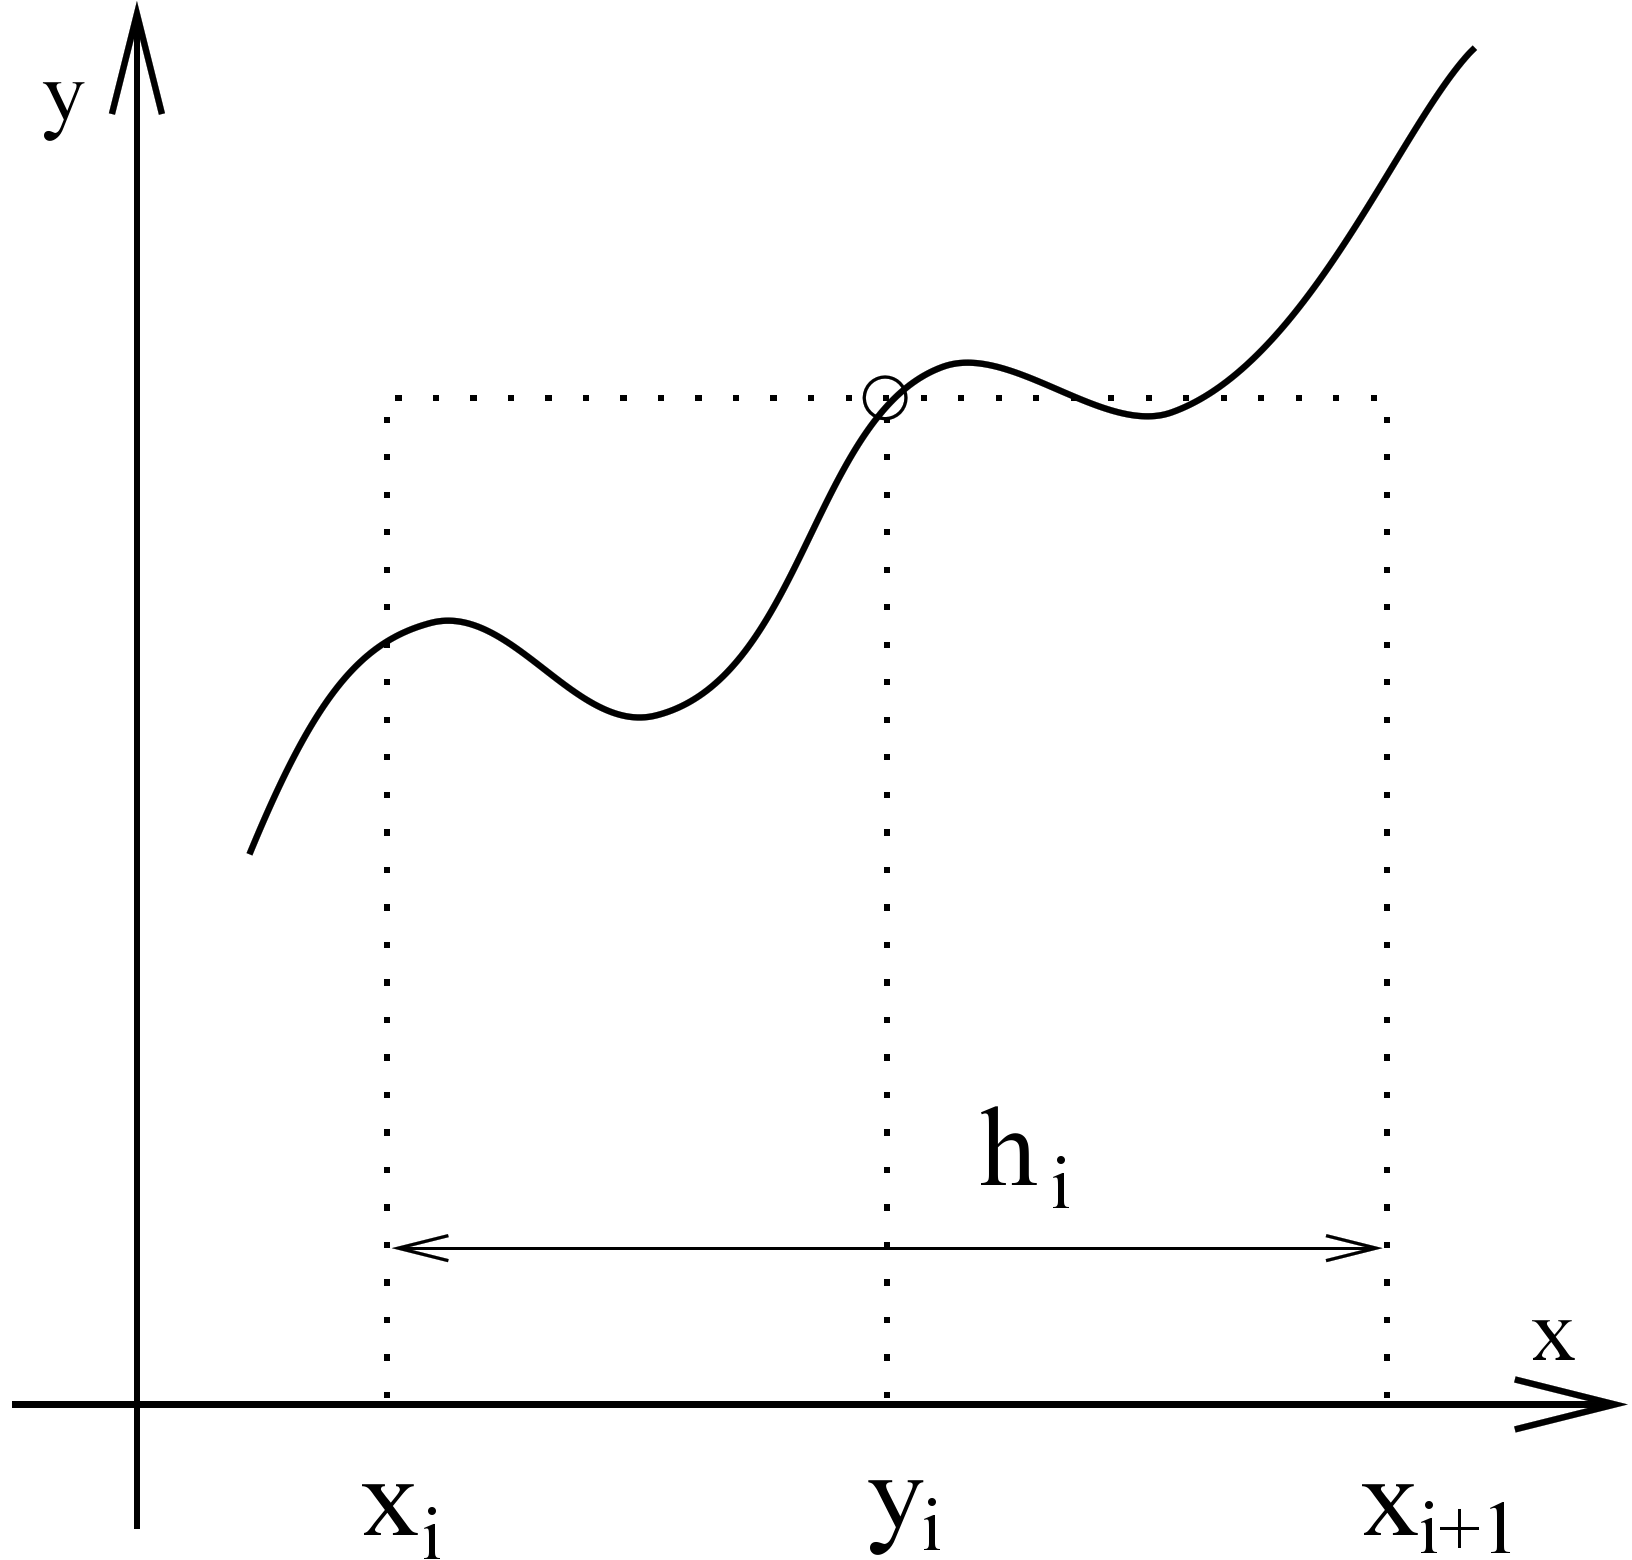
\includegraphics[width=0.4\linewidth]{img/6/image002.png}
      	\end{center}
     
      \textcolor{blue}{Idea:}
      $$
      	y_{i}= \frac{1}{2}(x_{i}+x_{i+1}),
      $$
      $$
      	\int_{x_{i}}^{x_{i+1}}f(x)dx \approx f(y_{i})h_{i}
      $$
	\end{frame}	
     \begin{frame}
     \textcolor{blue}{Własności:}
     \begin{itemize}
			\item stopień dokładności: 1
			\item kwadratura otwarta
    	\end{itemize}
    	$\newline$
    	\textcolor{blue}{Wyprowadzenie metody:}
		$$
f(x)=f(y_{i})+ \sum_{p=1}^{\infty}\frac{(x-y_{i})^{p}}{p!}f^{(p)}(y_{i})
		$$
        
		$$
\int_{x_{i}}^{x_{i+1}}f(x)dx=\underbrace{f(y_{i})h_{i}}_{R}+\underbrace{\frac{1}{24}h_{i}^{3}f''(y_{i})+\frac{1}{1920}h_{i}^{5}f^{(4)}(y_{i})+\ldots}_{blad \ metody}
		$$
	\end{frame}
%%%%%%%%%%%%%%%%%%%%%%%%%
	\begin{frame}{Wzór trapezów}
      \textcolor{blue}{Idea:}
      
      $$
      	\int_{x_{i}}^{x_{i+1}}f(x)dx \approx \frac{1}{2}[f(x_{i})+f(x_{i+1})]\cdot h_{i}
      $$
	
	\textcolor{blue}{Własności:}
     \begin{itemize}
			\item stopień dokładności: 1
			\item kwadratura zamknięta
    	\end{itemize}
    	$\newline$
    	\textcolor{blue}{Wyprowadzenie metody:}	 	
    	$$
f(x_{i})=f(y_{i})- \frac{1}{2}h_{i}f'(y_{i})+\ldots,\ \ f(x_{i+1})=f(y_{i})+ \frac{1}{2}h_{i}f'(y_{i})+\ldots
        $$
        
		$$
\int_{x_{i}}^{x_{i+1}}f(x)dx=\underbrace{\frac{1}{2}[f(x_{i}) + f(x_{i+1})] \cdot h_{i}}_{T} \underbrace{- \frac{1}{12}h_{i}^{3} f''(y_{i})-\frac{1}{480}h_{i}^{5}f^{(4)}(y_{i})+\ldots}_{blad \ metody}
		$$ 
	\end{frame}
%%%%%%%%%%%%%%%%%%%%%%%%%
	\begin{frame}{Wzór Simpsona}
	\begin{center}
      		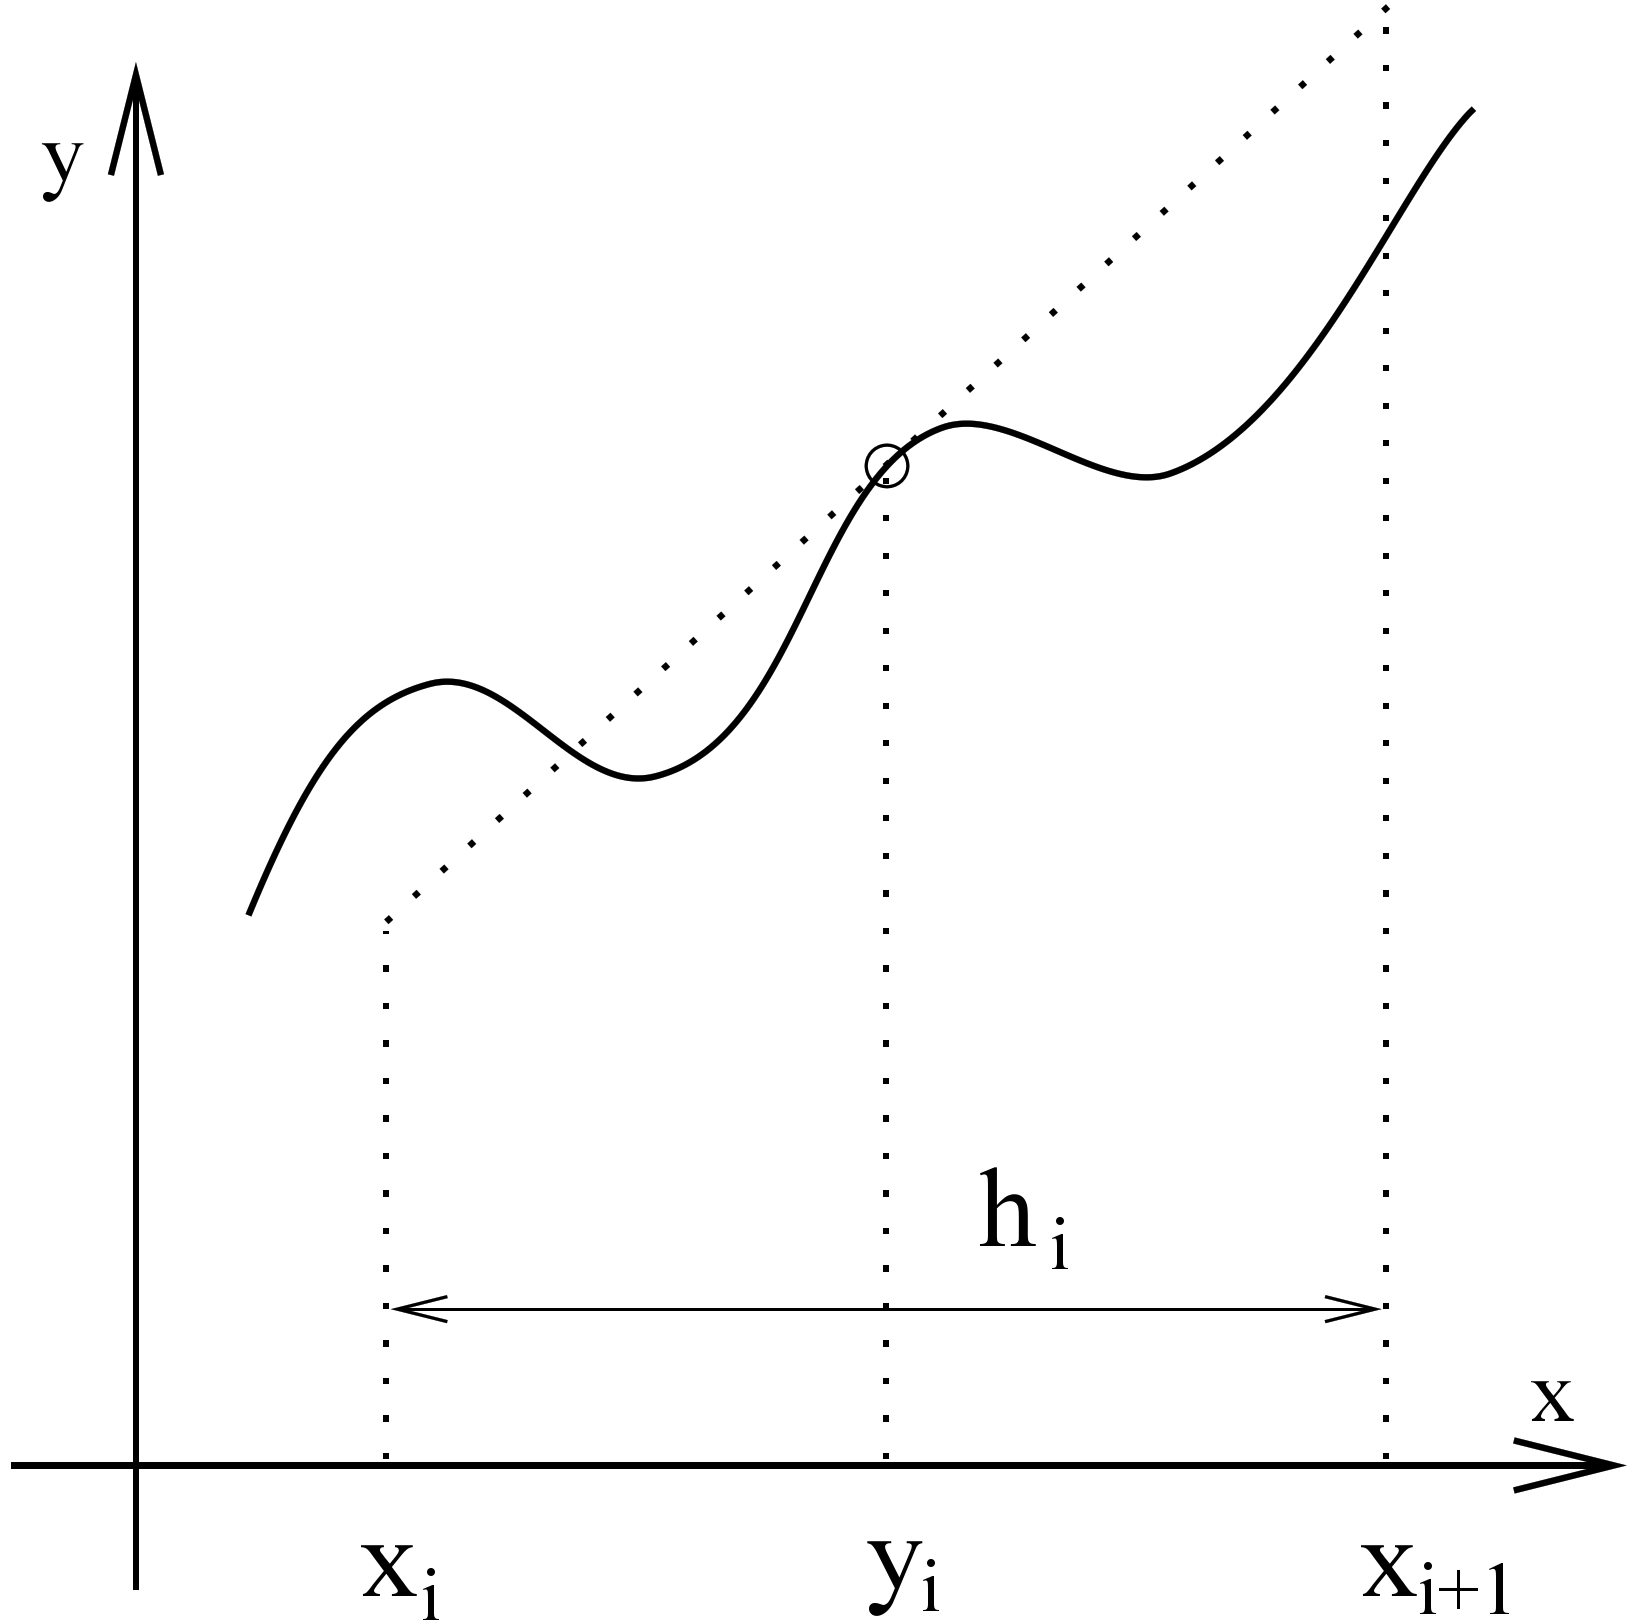
\includegraphics[width=0.4\linewidth]{img/6/image003.png}
      	\end{center}
      	$\newline$
      	Złożenie metody prostokątów i trapezów.
      	$$
        \textnormal{Sposób składania:} \left\{\begin{array}{l}
  			I = R + E + F \\
        	I = T - 2E - 4F
        \end{array}\right.
        $$
        
      	\end{frame}
      	
      \begin{frame}	
		\textcolor{blue}{Idea:}

        $$
\int_{x_{i}}^{x_{i+1}}f(x)dx \approx  \frac{1}{6}h_{i}[f(x_{i})+4f(\frac{x_{i}+x_{i+1}}{2})+f(x_{i+1})]
		$$
		$\newline$
		\textcolor{blue}{Błąd metody:}
		$$
		 \tilde{E}=-\frac{1}{2880}h_{i}^{5}f^{(4)}(y_{i})
		$$
		$\newline$
		\textcolor{blue}{Uwaga:}$\newline$
        Wzór Simpsona oparty na interpolacji 2-go rzędu, ale dokładny dla funkcji sześciennych.
        
      	
	\end{frame}
%%%%%%%%%%%%%%%%%%%%%%%%%
